\documentclass[border=10pt]{standalone}

\usepackage{tikz}
\usepackage{tikzsymbols}
\usetikzlibrary{calc,patterns,shapes.geometric}

\def\centerarc[#1](#2)(#3:#4:#5){\draw[#1] ($(#2)+({#5*cos(#3)},{#5*sin(#3)})$) arc (#3:#4:#5);}

\begin{document}
	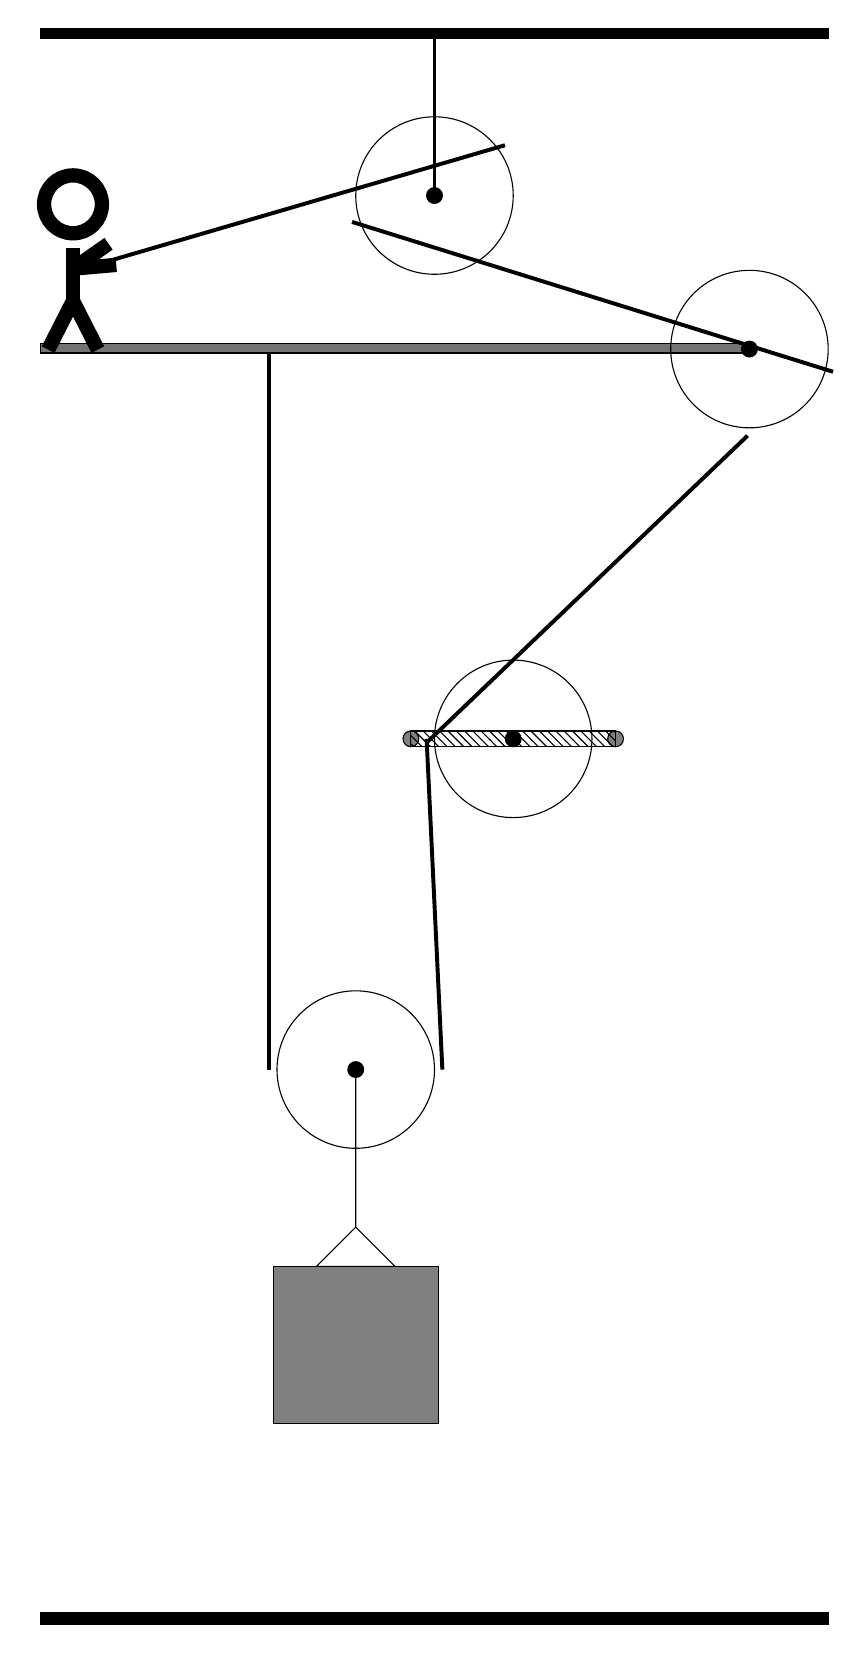
\begin{tikzpicture}
		%%%%% START %%%%%
		\draw[fill=black] (-2, 18) rectangle (8, 18.125);
		
		\draw[fill=black!55] (-2, 14) rectangle (7, 14.125);
		
		\draw (2, 4.9) circle (1);
		\draw[fill=black] (2, 4.9) circle (0.1);
		
		\draw (7, 14.05) circle (1);
		\draw[fill=black] (7, 14.05) circle (0.1);
		
		\draw[fill=white](4, 9.1) circle (1);
		\draw[fill=black] (4, 9.1) circle (0.1);
		\draw[fill=black!50] (2.7, 9.1) circle (0.1);
		\draw[fill=black!50] (5.3, 9.1) circle (0.1);
		\draw[pattern=north west lines, pattern color=black] (2.7, 9.2) rectangle (5.3, 9.0);
		
		\draw (3, 16) circle (1);
		\draw[fill=black] (3, 16) circle (0.1);
		\draw[line width=0.5mm] (3, 16) -- (3, 18);
		
		\draw (2, 4.9) -- (2, 2.9) -- (1.5, 2.4) -- (2.5, 2.4) -- (2, 2.9);
		\draw[fill=black!50] (0.95, 2.4) rectangle (3.05, 0.4);
		
		\draw[line width=0.5mm] (0.9, 14) -- (0.9, 4.9);
		\centerarc[line width=0.5mm](2, 4.9)(180:360:1.1);
		\draw[line width=0.5mm](3.1, 4.9) -- (2.9, 9.1);
		\centerarc[line width=0.5mm](4, 9.1)(110:180:1.1);
		\draw[line width=0.5mm](2.901, 9.052) -- (6.976, 12.95);
		\centerarc[line width=0.5mm](7, 14.05)(-60:50:1.1);
		\draw[line width=0.5mm](8.062, 13.762) -- (1.953, 15.665);
		\centerarc[line width=0.5mm](3, 16)(60:120:1.1);
		\draw[line width=0.5mm](3.895, 16.639) -- (-1.2, 15.15);
		
		\node at (-1.5, 15.15) {\Strichmaxerl[10][-175][35]};
		
		\draw[fill=black] (-2, -2) rectangle (8, -2.15);
		%%%%% END %%%%%
	\end{tikzpicture}
\end{document}